\documentclass{scrartcl}

\usepackage{amssymb}
\usepackage{amsmath}
\usepackage[dvipsnames]{xcolor}
\usepackage{tikz}
\usetikzlibrary{calc}	%for centerarc

\def\centerarc[#1](#2)(#3:#4:#5)% Syntax: [draw options] (center) (initial angle:final angle:radius)
{ \draw[#1] ($(#2)+({#5*cos(#3)},{#5*sin(#3)})$) arc (#3:#4:#5); }

\begin{document}
	
	%\begin{figure}
	%	\centering
	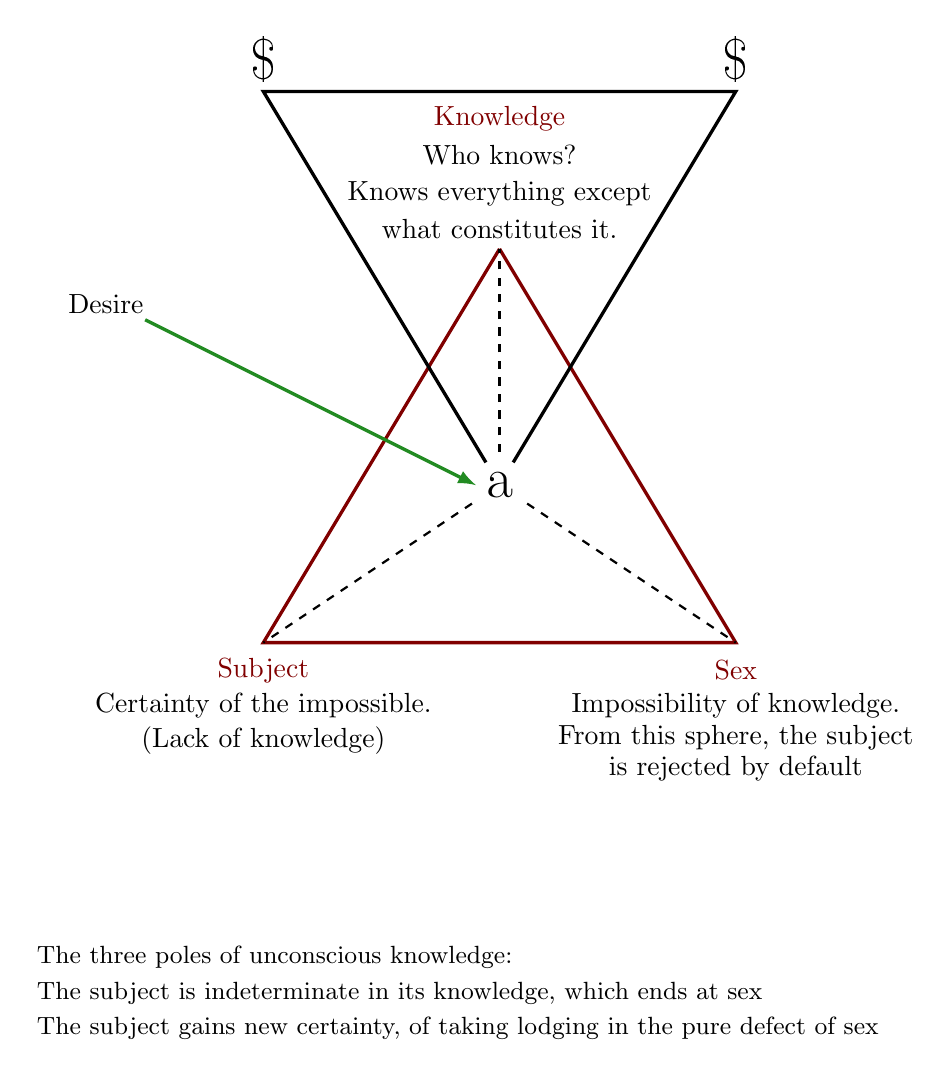
\begin{tikzpicture}
	\draw[very thick,Maroon] (0,3)--(-3,-2)--(3,-2)--(0,3);	%red triangle
	\draw[thick,dashed] (0,0)--(0,3);
	\draw[thick,dashed] (0,0)--(-3,-2);
	\draw[thick,dashed] (0,0)--(3,-2);
	\draw[very thick] (0,0)--(-3,5)--(3,5)--(0,0);			%black triangle
	
	\centerarc[black,very thick](0,3.2)(-65:245:3)	%top circle
	\centerarc[black,very thick](-3,-2)(60:365:3)	%left circle
	\centerarc[black,very thick](3,-2)(-185:120:3)	%right circle
	
	\node[circle,draw=white,fill=white,inner sep=2pt,minimum size=5.5pt] (a) at (0,0) {\huge a};
	\node at (-3,5.4) {\huge \$};
	\node at ( 3,5.4) {\huge \$};
	\draw[very thick,->,>=latex,ForestGreen] (-4.5,2.1)--(-0.3,0);		%(-1.7,0.7)
	\node at (-5,2.3)  {Desire};
	%
	\node at (-3,-2.35)  {\textcolor{Maroon}{Subject}};
	\node at (-3,-2.8)  {Certainty of the impossible.};
	\node at (-3,-3.25) {(Lack of knowledge)};
	%
	\node at  (3,-2.35)  {\textcolor{Maroon}{Sex}};
	\node at  (3,-2.8)  {Impossibility of knowledge.};
	\node at  (3,-3.2)  {From this sphere, the subject};
	\node at  (3,-3.6)  {is rejected by default};
	%
	\node at (0,4.65) {\textcolor{Maroon}{Knowledge}};
	\node at (0,4.2)  {Who knows?};
	\node at (0,3.7) {Knows everything except};
	\node at (0,3.25) {what constitutes it.};
	
	\node[align=left,right] at (-6,-6)    {\small The three poles of unconscious knowledge:};
	\node[align=left,right] at (-6,-6.45) {\small The subject is indeterminate in its knowledge, which ends at sex};
	\node[align=left,right] at (-6,-6.9)  {\small The subject gains new certainty, of taking lodging in the pure defect of sex};
	\end{tikzpicture}
	%	\caption{...}
	%\end{figure}
	
\end{document}